%========================%
%        Preamble        %
%========================%
\documentclass[12pt]{amsart}

    %========================%
%        Packages        %
%========================%

\usepackage[utf8]{inputenc}
%\usepackage{amsmath}    % Included in amsart package
%\usepackage{amsthm}     % 
\usepackage{amssymb}      % 
\usepackage{mathtools}      % Paired Limiter Macros
% \usepackage{mdframed}       % boxes for theorem
\usepackage{enumitem}     % Continuous numbering of lists
\usepackage[hidelinks]{hyperref}
\usepackage{tikz}
\usetikzlibrary{positioning}
\usepackage{blindtext}
\usepackage{graphicx}
\usepackage{float}

%========================% 
%          Title         %
%========================% 
\title{Lecture 7 and 8}
\author{Anish Sundaram}
\date{\today}

%========================% 
%        Theorems        %
%========================% 
\theoremstyle{definition}
\newtheorem{theorem}{Theorem}  % Boxed theorems
\newtheorem{definition}{Definition} % Definitions
\newtheorem{example}{Example}       %
\newtheorem{algorithm}{Algorithm}
\newtheorem*{proof*}{Proof}         % non-numbered
\newtheorem*{remark}{Remark}        %
\numberwithin{equation}{theorem}    % Local equation numbering

\setcounter{tocdepth}{3}      % Show subsubsections in contents

%========================% 
%        Macros          %
%========================% 
\DeclarePairedDelimiter\abs{\lvert}{\rvert}  % Vertical bars
\DeclarePairedDelimiter\norm{\lVert}{\rVert} % Double vertical bars
\newcommand{\drawvec}[1]{                    % matrices on one line
    \begin{bmatrix}
        #1
    \end{bmatrix}
}


% \begin{figure}[H]
%     \centering
%     \includegraphics[width=5in]{global-carbon-cycle.png}
%     \caption{The Global Carbon Cycle}
%     \label{global-carbon-cycle}
% \end{figure}

%========================% 
%         Document       %
%========================% 
\begin{document}

\maketitle

\tableofcontents

\section*{7 Jointly Distributed Random Variables}
\subsection*{7.1 JDRV Discrete Case}


\begin{definition}
    \textbf{JDRV}:
    Can be described as the computation $$\mathcal{P}{(X,Y) \in B}$$
    for all possible sets.
    \begin{remark}
        Summing across all values x and y will result in 1 and the probability of p(x,y) must at least be 0.
    \end{remark}
\end{definition}

\subsection{7.2 Marginal Distributions}


\begin{definition}
    \textbf{Marginal Distributions}:
    The probability distribution of the variables contained in the subset. Can be found using the equation $$p_Y(y) = \sum{_x}p_{X,Y}(x,y)$$. Suppose we roll a pair of dice and let X be the minimum and Y the maximum of the two scores:
    The conditional PMF of $Y$ given $X = x_0$ is defined as:
    $$p_{Y|X} : = P[Y=y|X=x_0] = \frac{p_{X,Y}(x_0,y)}{p_x(x_o)}$$

\end{definition}

\subsection*{7.2 Conditional Distributions}

\begin{definition}
    \textbf{Conditional Distribution}:
    A probability distribution for a sub-population. In other words, it shows the probability that a randomly selected item in a sub-population has a characteristic you’re interested in. 

\end{definition}


\begin{figure}[H]
    \centering
    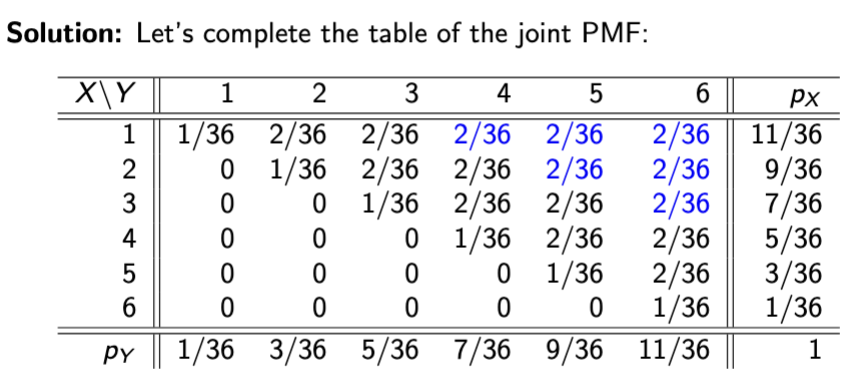
\includegraphics[width=3in]{Media/jointdist.png}
    \caption{Example of a Joint Distribution}
    \label{joint distribution}
\end{figure}


\section*{8 Jointly Distributed Randvars}

\subsection*{8.1 Covariance}

\begin{definition}
    \textbf{Covariance}:
    Defined as the measure of joint variability of two random variables. Do they trend together or inversely?At all?
    Covariance of 2 random variables X and Y is defined as $$Cov(X,Y) = E[(X-\mu_x)(Y-\mu_y)]$$ where $$\mu_x = E[X]$$ and $$\mu_y = E[Y]$$ are the means of $X$ and $Y$ respectively and can also be seen as 
    $$\frac{1}{n}\sum_{i=1}^{n}(X_i - \bar{X_n})(Y_i-\bar{Y_n})$$ for population and $$\frac{1}{n-1}\sum_{i=1}^{n}(X_i - \bar{X_n})(Y_i-\bar{Y_n})$$ for samples
\end{definition}

\begin{definition}
    \textbf{Properites of Covariance}:
    Covariance is sensetive to scale, and has various properties:
    \begin{enumerate}
        \item Symmetry: $Cov(X,Y) = Cov(Y,X)$
        \item Linearity: 
        \item If X and Y are independent then $Cov(X,Y) =0$
    \end{enumerate}
\end{definition}


\subsection*{8.2 Correlation Coefficient}

\begin{definition}
    \textbf{Correlation Coefficient($\rho)$}:
    A unitless statistical measure of the strength of the relationship between the relative movements of two random variables. Defined mathematically as:
    $$Corr(X,Y) = \frac{Cov(X,Y)}{\sigma_X\sigma_y} =
    \frac{\sum (X_i - \bar{X_n})(Y_i-\bar{Y_n})}{\sqrt{\sum x_i - \bar{x})^2\sum (y_i - \bar{y})^2)}}$$
\end{definition}



\begin{theorem}
    \textit{Cauchy-Schwarts}:

\end{theorem}

\subsection*{8.3 Density of Transformation}


\subsection*{8.3 Transformations of RVs}

\begin{definition}
    \textbf{linear}
\end{definition}



\begin{definition}
    \textbf{nonlinear}
\end{definition}
\end{document}